\section{Control of physics-based animation}

\subsection{Context}
As we mentionned in the introduction, computer helped in producing animations in two ways. First, principles of traditional animation have been adopted, leaving the animator to describe the keyframes that would bring life and style to characters. Second, physics has been used to animate objects whose complexity in terms of scale and behavior would have been intractable for a single animator. However, they are only the extremities of a large spectrum. In between lie the control of physics-based animation which tends to take into account both user directions, that will bring life and style, and physics, that will handle the exciting complexity of the physical behavior.

\subsection{Problems: The trials and errors process}

How to control a physics-based animation is an old problem in Computer Graphics. In order to understand the different problems that arise, it is good to start from the most naive way of controlling a physics-based animation: trials and errors. 

Let's say we have to design an animation of a ball launched on the ground that bounces two times before hitting the center of a target on the ground. The elastic behavior of the ball make it a hard animation for a key-framing animator. For physics, the behavior takes some time to compute but it can be solved.

As the simulation is an initial value problem, the whole behavior of the ball is dictated by the initial and boundary conditions of the simulation, the material parameters of the ball and the \emph{wind} forces that can be set to help guiding the animation. The trials and errors process consists in setting these conditions and parameters, running the simulation and correcting the parameters until the animation is fine (see Figure~\ref{fig:trialErrorProcess}. There are mainly two constraints which make this task a nightmare.

\begin{figure}[!h]
\centering
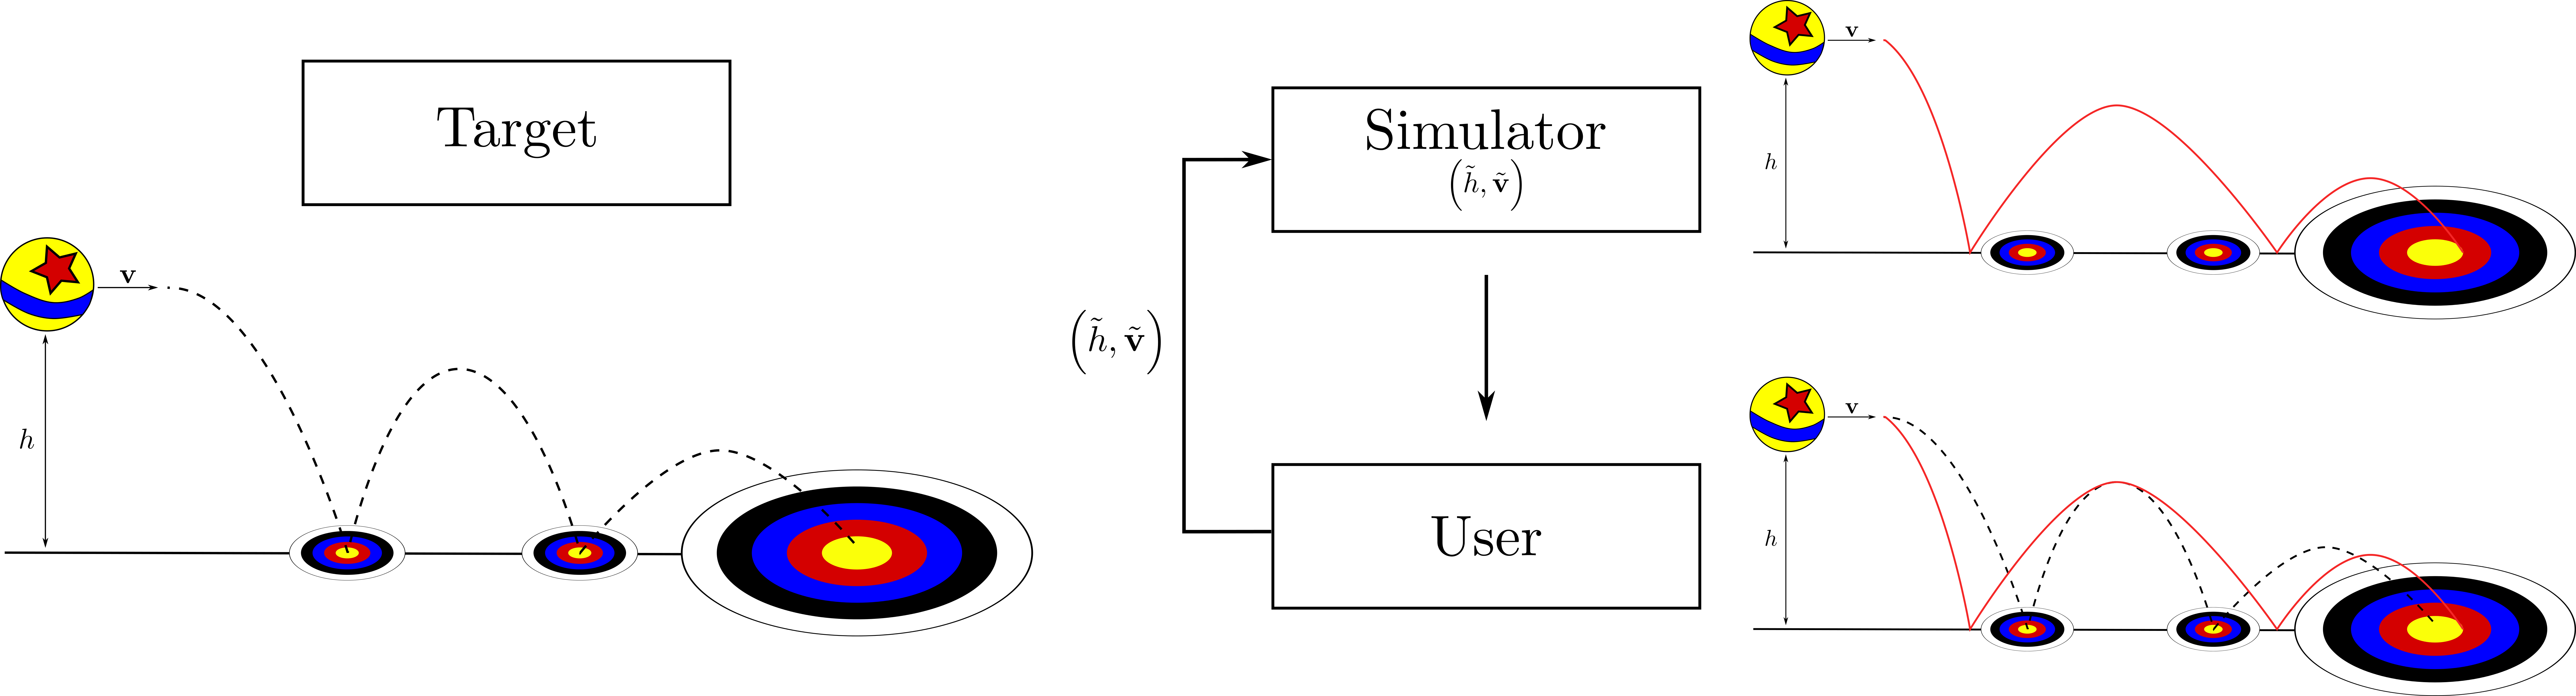
\includegraphics[scale=0.20]{./images/simulationControl/trialError.png}
\caption[STAR control: Trial and error process]{\label{fig:trialErrorProcess}Trial and error process}
\end{figure}

First, the computational time plays a major role. This is obvious but still important to states. A real-time simulation will allow the user to quickly explore parameters whereas an offline simulation might require days and days of tuning.

Second, the nonlinear behavior of most physics-based animation makes it very hard to choose the right parameters. Small changes can produce very different results making tedious to explore the range of possible behaviors and almost impossible to respect specific artistic directions such as timing, key positions, trajectories or shapes. Also, it prevents the user from running a low resolution simulation in real-time and then run an offline high resolution simulation with the same parameters.

\subsection{Space-time constraints paradigm}
A general approach for controlling a physics-based animation is to formulate it as an optimization under constraints: "Find the parameters such that the physical behavior and user constraints are respected over the animation" ((see Figure~\ref{fig:spaceTimeConstraints}. Four challenges arise, what are the parameters we want to control, what are the user constraints, how to formulate them and finally how to numerically solve the problem. Witkin and Kass~\cite{Witkin1988} were among the first to introduce this formulation to the Computer Graphics community in their work \emph{Spacetime constraints}.

\begin{figure}[!h]
\centering

\includegraphics[scale=0.20]{./images/simulationControl/spaceTimeConstraints.png}
\caption[STAR control: Space-time constraints]{\label{fig:spaceTimeConstraints} Space-time constraints}
\end{figure}

\subsubsection{Parameters}
Most common parameters are the position of the degrees of freedom and the \emph{wind} forces. A common drawback of using \emph{wind} forces is that they can create non-physical behavior. As an alternative, Coros et al.~\cite{Coros2012} proposed to adapt the rest shape of the object from one frame to another in order to induce internal forces that would match the user goals. When large deformation occurs it is possible that the found solution it at the limit of the deformation that the object can reach. In order to enforce the optimization, Li et al.~\cite{Li2014} proposed to optimize material parameters as well. 

\subsubsection{Constraints}
Position, velocity, density are among the constraints that are often used for controlling an animation. Of course they depend on the simulated object: rigid, solids, smoke, liquid, $\dots$. Certainly, position constraints are the most intuitive for the user as they can be specified by keyframes. Howevever, designing a keyframe for a highly elastic object might be tedious. Here there is a direct link to the works about surface modeling which propose to deform naturally an object \cite{Sorkine2007, Hildebrandt2011}. In some cases, these deformation tools can be seen as a local static simulation of the object that computes its deformation from a position change induced by the user. For elastic objects and fluids, such deformation tool have been proposed respectively by Barbic et al. \cite{Barbic2012} and Pan et al. \cite{Pan2013}. Both fits in the framework of surface modeling deformation. The only difference is that the function which are minimized are directly derived from the internal forces acting on the object. These methods are particularly useful when interactively editing an animation, specially when they are combined with high level deformation tool such as sketching.

\subsubsection{Numerical solving}
In their work, Witkin and Kass~\cite{Witkin1988} dealt with small systems on short simulation time. Therefore they could afford to directly solve the optimization problem, meaning that at each iteration a whole simulation would be computed. For instance, small rigid bodies simulation could be interactively designed through this approach \cite{Popovic2000},\cite{Popovic2003}. For complex models and large simulation time, this approach tends to take forever. Windowing methods allowed to restrict the optimization to the space-time range of interests \cite{Cohen1992}. In their work \cite{McNamara2004} proposed to use the adjoint method to efficiently compute gradients in liquid simulation thus improving the performance of the optimization. The approach was also used by Wojtan et al.~\cite{wojtan2006keyframe} for handling large particle systems. For elastic bodies, the use of reduced model allowed to achieve speed-ups of several order of magnitude, thus allowing to interactively edit a physics-based animation~\cite{Barbic2012},\cite{Hildebrandt2012}, \cite{Hahn2012}. Since, this approach has been further improved to be faster \cite{Schulz2014} and deal with large deformations \cite{Li2014}.

\subsection{Applications \& Alternatives}
The strength of the space-time constraints paradigm relies on its very general definition. Therefore, a large number of applications and methods can be seen as offsprings of this approach. In the following, we distinguished different applications of physics-based animation control and present alternatives to the above methods.

\subsubsection{Enriching an animation with physics}
Given a full animation, a simulation is run in order to enhance the input animation with detailed physically-based secondary motions. This approach was successfully applied to enhance character animation with wrinkles and folds of their skin by Bergou et al.~\cite{Bergou2007}. In their work, they compute the dynamics of thin shells on top of the animation by using a multi-resolution approach. In fluid animation, details enhancing brings a lot of attention as it would be easier to set up low resolution simulation and add details on top of it without loosing the global behavior. A nice approach was proposed by Mercier et al. \cite{Mercier2015} where they solve a Lagrangian wave simulation only at the surface of the low resolution simulation.

\subsubsection{Guiding a high resolution simulation with animation}
A large number of methods propose to guide a simulation without the need of an expensive optimization problem. Generally these methods propose to use external forces that are automatically computed from the user inputs such as keyframes or more involved data such as velocity and density field. Another proposed strategy is to use a low resolution simulation to guide a high resolution one. Thus, correct parameters can be found in a real-time simulator and be re-used for the high resolution simulation.  We details such methods in the context of fluid simulation control in section~\ref{subsec:fluidControl}

\subsubsection{Example-based simulation}
Instead of controlling the trajectory of an object, one might want to control how it deforms when it collides with other objects. In exampled-based simulations, a set of examples that represent the desired deformations is used to build a space of preferred deformations from where internal forces will be deduced. This method was first introduced by Martin et al.~\cite{Martin2011} for elastic deformations. Jones et al.\cite{Jones2016} propose a similar method to easily incorporate plastic deformations in rigid bodies simulations.

\subsubsection{Animation sampling}
In multibody systems, space-time constraints paradigm can hardly be used. In cause, the large number of discontinous contacts events which make the optimization problem particularly difficult to solve. In contrast, multibody simulators are particularly fast, so fast that it is possible to run in parallel a large number of simulations. In their work, \cite{Chenney2000} and \cite{Twigg2007} exploit this performance to sample the space of parameters of an animation and thus finding those which satisfy the user constraints.

\subsubsection{Animation editing} 
In constrast with simulation control, animation editing consists in deforming in space and time the output of a simulator. Closely related to surface modeling it has to take into account the temporal dimension and its relation with space in order to propose new editing tools. Very few methods have been proposed whereas modifying the result of a simulation frame by frame is a common practice in animation studios. Among the most interesting approach, Pighin et al.\cite{Pighin2004} propose to build a space-time parameterization of a smoke animation using radial basis function. In these approaches, finding a natural way to deform an animation and ensuring temporal coherency are amongst the main challenges. For liquid animations, Raveendran et al.~\cite{Raveendran2014} match two liquids animations and propose a method to smoothly blend between them. This approach allows to quickly explore parameter space such as boundary conditions or viscosity parameter and then to produce a large number of new liquid animations whithout the need to re-simulate.

\subsection{Control of fluid simulation}
\label{subsec:fluidControl}
In this section we focus on the control of fluid simulation.

The standard pipeline for controlling a simulation is mainly based on trial and error. Fluid parameters and boundary conditions are first set up by the user. The parameters are then tweaked and the simulation is re-run until reaching the expected behavior. The control is indirect, for instance the user cannot control the trajectory nor the shape of the fluid. Moreover, the non-linear nature of the fluid behavior prevents the user from interactively controlling a low-resolution simulation and then achieving similar behaviors with the same parameters at a higher resolution.

To overcome these limitations, several methods propose to guide the fluid behavior by using geometric proxies which are easier to control than the high resolution fluid simulation variables themselves.
For example, artists can use a triangle mesh to specify a target shape for the fluid by adding artificial attraction forces based on the distance to the mesh surface. Similar approaches have been successfully developed to drive smoke~\cite{Fattal2004,Hong2004,Shi2005a} and liquid simulations~\cite{Shi2005b,Raveendran2012}. These meshes can also define specific keyframes from a global animation~\cite{Treuille2003,McNamara2004}.
Fluid trajectories can also be controlled with user-defined velocity fields~\cite{Kim2006}, distance fields~\cite{Yang2013}, or specific control particles~\cite{Thurey2006,Madill2013}. 

Taking this strategy further, the attracting surface itself can defined by a low-resolution fluid simulation. To achieve this, the artist quickly sets up a coarse simulation and uses the output geometry to guide the main features of a full resolution simulation.
Several approaches modify a high-resolution smoke simulation using optimization~\cite{Nielsen2009,Nielsen2010}, patterns extracted as skeleton~\cite{Yuan2011}, or sparse sampling~\cite{Huang2013}.
For liquid simulations, Nielsen and Bridson~\cite{Nielsen2011} propose to restrict the high resolution simulation to a thin layer around a guiding coarse animation.

Although each of these approaches are able to successfully guide a fluid simulation, they do not enable direct control of the resulting fluid. Designing precise timing or feature scaling would therefore still require iterative trial-and-error steps to converge toward a desired animation.
Few attempts have been made to enable direct control on the simulation. Schpok et al.~\cite{Schpok2005} proposed to extract and parameterize features such as vortices, uniform advection, sinks, and sources to allow the user to modify the parameters in a smoke simulation. In the context of liquid simulation, Pan et al.~\cite{Pan2013} propose a method to deform wave shapes by sketching their profiles. This approach enables direct spatial deformation but does not allow temporal editing, and the simulation needs to be re-computed from the modified frame onwards.

Editing fluid animation is usually handled through indirect control, by adjusting physically based simulation parameters and degrees of freedom~\cite{stam1999,ihmsen2014}, or by editing control parameters of procedural generation models for ocean and waves~\cite{Fournier1986,hinsinger2002,Tessendorf2004,jeschke2015water}. 

%Direct editing of simulation has been addressed in the contexts of rigid bodies and of deformable objects~\cite{Chenney2000,wojtan2006keyframe,Twigg2007,Barbic2009,Barbic2012,Schulz2014,Li2014}, but only few works have focused on fluid surfaces, due to the fact that the constantly changing shape and topology makes the output geometry inaccessible to standard deformation tools.
%Interactvity and intuitivity, \cite{Kondo2005}
%\begin{itemize}
%\item It is tempting to create tools that allow a higher level of control on the design of a physics-based animation.
%\end{itemize}
